\documentclass[12pt]{article}
\usepackage[utf8]{inputenc}
\usepackage[dvipsnames]{xcolor}
\usepackage[leqno]{amsmath}
\usepackage{amssymb}
\usepackage{units}
\usepackage{wallpaper}
\usepackage{newtons-notebook}
\usepackage{booktabs}
\usepackage{float}
\usepackage{xurl}
\usepackage{listings}
\usepackage{tocloft}
\usepackage{setspace}
\usepackage{titlesec}

\titlespacing\section{0pt}{12pt plus 4pt minus 2pt}{0pt}
\titlespacing\subsection{0pt}{12pt plus 4pt minus 2pt}{0pt}
\titlespacing\subsubsection{0pt}{12pt plus 4pt minus 2pt}{0pt}

\renewcommand{\cftpartfont}{\Large\bfseries}
\renewcommand{\cftsecfont}{\normalsize}

\setlength{\parskip}{\baselineskip}
\renewcommand{\baselinestretch}{1.5}

\addtolength{\oddsidemargin}{-.25in}
\addtolength{\evensidemargin}{-.25in}
\addtolength{\textwidth}{0.5in}
\addtolength{\topmargin}{-.25in}
\addtolength{\textheight}{0in}

\begin{document}
\setcounter{tocdepth}{1}

%\nnimagepage{Title_Page_2019.pdf}

\begin{figure}[H]
    \centering 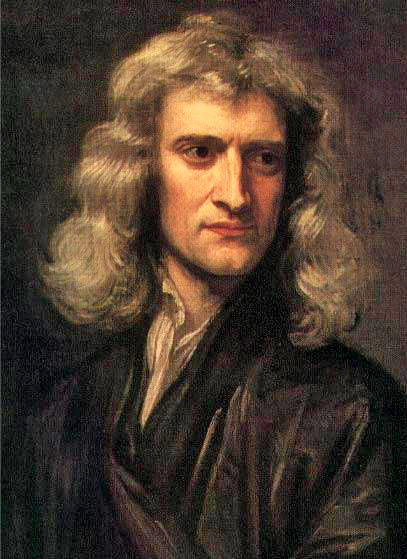
\includegraphics[scale=1]{newton.jpg}
    \\
    \textbf{\large{``To explain all nature is too difficult a task for any one man or even for any one age. `Tis much better to do a little with certainty and leave the rest for others that come after you.'' --Isaac~Newton}}
\end{figure}

\nnwallpaper{2020_Intro_Section_Page_Border.pdf}

\begin{spacing}{1.0}
\tableofcontents
\end{spacing}

\newpage
\subsection*{Mission Statement}
\textit{Newton’s Notebook: The Haverford School STEM Journal} is designed to enhance the interests, talents, and achievements of individuals in mathematics and science and to promote the work of those most passionate about these disciplines. The following articles were written by members and friends of the Haverford community and edited by the \textit{Notebook staff}. We hope these articles inspire readers to further discover the universally beautiful realm of STEM exploration. 
\subsection*{Staff}
{\centering{}
    \textbf{Editor-in-Chief:} Alexander Greer '20
    \\
    \textbf{Assistant Editors:} Gary Gao '21, Mitav Nayak '22, Safa Obuz '21, Shibo Zhou '22
    \\
    \textbf{Designer-in-Chief:} Alexander Greer
    \\
    \textbf{Faculty Advisor:} Dr.\ Mark Gottlieb
    \\}
\subsection*{Featured Polymath: Richard Phillips Feynman (1918-1988)}
Richard Phillips Feynman was an American theoretical physicist known for his work on quantum mechanics, quantum electrodynamics, and particle physics. Born in Queens, New York, in 1918, Feynman excelled in math and science in high school. He attended the Massachusetts Institute of Technology and graduated with a bachelor’s degree in physics in 1939. In early 1943, Feynman was recruited by Robert Oppenheimer to work as a researcher on the Manhattan Project developing the atomic bomb. Soon after his work, Feynman took up a position as a physics professor at Cornell University. There he developed Feynman diagrams, a system of visually representing mathematical expressions describing the interaction of subatomic particles. In 1951, Feynman took up a position at the California Institute of Technology after taking a year-long sabbatical in Brazil. At Caltech, Feynman explored superfluidity and superconductivity, as well as conceiving the possibility of quantum computers. In the early 1960’s, Feynman produced \textit{The Feynman Lectures on Physics}, a lecture series outlining undergraduate physics concepts still used by university students to this day. In 1965, Feynman and two colleagues were awarded the Nobel Prize in Physics for their work on quantum electrodynamics. Feynman’s contributions to the advancement of human knowledge are innumerable, and his legacy as one of the world’s most-renowned scientists lives on. 
\newpage

% Begin the pure math section
\addcontentsline{toc}{part}{Pure Mathematics}
\nnimagepage{Pure_Math_Title_Page.pdf}

\nnwallpaper{Pure_Math_Border.pdf}
\def\currentTitleWallpaper{Pure_Math_Border_Title.pdf}

\nnarticleheader{Squaring Prime Numbers}{Mickey Fairorth '19}

\subsection*{Conjecture}

The result of squaring any prime number \(P\) will result in a number that is one more than a multiple of 24, given that \(P > 3\).

\subsection*{Proof 1:}

The first step in this proof is to establish where prime numbers fall relative to other numbers. So let’s look at a number line and notice where all the primes are relative to other numbers:
\[1  \quad 2 \quad 3 \quad 4 \quad \textbf{5} \quad [6] \quad \textbf{7} \quad 8 \quad 9 \quad 10 \quad \textbf{11} \quad [12] \quad \textbf{13} \quad 14 \quad 15 \quad 16 \quad \textbf{17} \quad [18] \quad \textbf{19} \quad 20 \quad 21 \quad 22 \quad \textbf{23} \quad [24] \quad 25\]

*For this proof, 2 and 3 are subprimes and will not be regarded as prime.

Clearly, the primes are always one less or one more than a multiple of 6. This may seem puzzling at first but makes sense at second glance. Obviously, primes cannot be multiples of 6 because then they would not be prime. They also must not fall two above or below multiples of 6 because then they would be even and therefore have 2 as a factor. Finally, primes cannot be halfway between multiples of 6 because they would have 3 as a factor, so prime numbers must be directly above or below a multiple of 6. This does not imply that every number above or below a multiple of 6 is a prime, but that every prime must be above or below a multiple of 6. For example, the number 25 is one above 24 but is not prime. 

Now that we have established where the primes are located, we can represent them algebraically.


\[
    \begin{cases}
    P = 6k + 1, k \in \mathbb{Z} \\
    P = 6k - 1, k \in \mathbb{Z}
    \end{cases}
\]

Every k must be odd or even, which means \(k\) can be substituted for \(2m\) and \(2m +1\).

\[
  \begin{cases}
    P = 6(2m) + 1, m \in \mathbb{Z} \\
    P = 6(2m + 1) + 1, m \in \mathbb{Z}
  \end{cases} \Longrightarrow \begin{cases}
    P = 12m + 1, m \in \mathbb{Z} \\
    P = 12m + 7, m \in \mathbb{Z}
  \end{cases}
\]

\[
  \begin{cases}
    P = 6(2m) - 1, m \in \mathbb{Z} \\
    P = 6(2m + 1) - 1, m \in \mathbb{Z}
  \end{cases} \Longrightarrow \begin{cases}
    P = 12m - 1, m \in \mathbb{Z} \\
    P = 12m + 5, m \in \mathbb{Z}
  \end{cases}
\]

Now we have four equations that represent every possible prime. So, if we square these equations, we can show that every prime squared is one more than a multiple of 24.

\[
    \begin{cases}
        P^2 = {(12m + 1)}^2 \\
        P^2 = {(12m + 7)}^2 \\
        P^2 = {(12m - 1)}^2 \\
        P^2 = {(12m + 5)}^2
    \end{cases} \Longrightarrow \begin{cases}
        P^2 = 144m^2 + 24m + 1 \\
        P^2 = 144m^2 168m + 49 \\
        P^2 = 144m^2 - 24m + 1 \\
        P^2 = 144m^2 + 120m + 25
    \end{cases} \Longrightarrow \begin{cases}
        P^2 = 24(6m^2 + m) + 1 \\
        P^2 = 24(6m^2 + 7m + 2) + 1 \\
        P^2 = 24(6m^2 - m) + 1 \\
        P^2 = 24(6m^2 + 5m + 1) + 1
    \end{cases}
\]

Therefore, the square of every prime number is one more than a multiple of 24. 

Q.E.D.

\subsection*{Proof 2:}

This proof will come to the same conclusion but relies less on algebra and more on observations and patterns. By stating that the square of every prime number is one more than a multiple of 24, we also imply that one less than every prime squared is a multiple of 24.

\[P^2 - 1 = 24k, k \in \mathbb{Z}\]

This expression may seem familiar to the reader, not because of its meaning with prime numbers, but because it fits the form of the difference of two squares. This allows us to rewrite the expression.

\[(P + 1)(P - 1)\]

Now we have three integers to consider: \(P - 1\), \(P\), and \(P + 1\). These numbers obviously fall directly next to each other because they are separated by one. We know that every other number is a multiple of 2. This number cannot be \(P\) because \(P\) has no factors, so \(P - 1\) and \(P + 1\) are both even. From this, we know that our expression is a multiple of 4.

\[(P + 1)(P - 1) = 4m, m \in \mathbb{Z}\]

We also know that every other even number is a multiple of 4. It does not matter whether \(P - 1\) or \(P + 1\) is a multiple of four, but this allows us to now state that our expression is a multiple of 8. 

\[(P + 1)(P - 1) = 8k, k \in \mathbb{Z}\]

The final piece of the puzzle relies on multiples of 3. Out of three numbers in a row, one of the numbers must be a multiple of 3. This number cannot be \(P\) because then \(P\) would not be prime, so either \(P - 1\) or \(P + 1\) is a multiple of three. So, besides being a multiple of 8, our expression must also be a multiple of 3 which lands us at our conclusion.

\[P^2 - 1 = 24k, k \in \mathbb{Z}\]

The square of any prime number is one greater than a multiple of 24.

Q.E.D.


\newpage

\nnarticleheader{The Law of Large Numbers}{Chris Tsetsekos '20}

In probability theory, the Law of Large Numbers (LLN) is a theorem that describes the result of performing the same experiment a large number of times. According to the law, the average of the results obtained from a large number of trials should be close to the expected value, and will tend to become closer as more trials are performed.

The LLN is important because it guarantees stable long-term results for the averages of some random events. For example, while a casino may lose money on some spins of the roulette wheel, it will have predictable earnings over a large number of spins. Any winning streak by a player will eventually be overcome by the parameters of the game. It is important to remember that the law only applies (as the name indicates) when a large number of observations is considered. There is no principle that a small number of observations will coincide with the expected value or that a streak of one value will immediately be "balanced" by the others, which are ideas collectively referred to as the “Gambler’s Fallacy”.

This past spring, I won 197 faceoffs out of 324 attempts for The Haverford School lacrosse team. This translates to a 60.8\% success rate. This past summer, I went 339-for-552. I took 228 more faceoffs in the summer than the spring; however, my success rate remained nearly identical: 61.4\%. This small difference – eight tenths of a percent – is a good example of the Law of Large Numbers: no matter how many faceoff attempts I take, it is highly likely that my success rate will be the same. 


\newpage

\nnarticleheader{The Search for New Primes}{Safa Obuz '21}

The study of prime numbers, a specific yet important branch of study in number theory, continues as a researched topic dating back from 2000 years ago and holds itself in increasing importance during the last century and into the future. Simply put, all of the modern world’s cryptography is based in our collective understanding of primes and their behavior. 

\subsubsection*{What is a Prime?}

A prime number is a natural number larger than 1 which cannot be expressed as the product of two smaller natural numbers. 
\[2, 3, 5, 7, 11, 13, 17, 19, 23, 29, 31, 37, 41, 43, 47, 53, 59 ,61, 67, 71, 73, 79, \ldots \]
They are effectively the analog of “atomic elements” of natural number multiplication. This comes from the one of the first theorems of primes.

\textbf{Fundamental theorem of arithmetic:}  (Euclid, \(\approx 300\) BCE) Every natural number larger than 1 can be expressed as a product of one or more primes. This product is unique up to rearrangement.

Other than the trivial rearrangement of the multiplication of primes, for instance, 50 can be \(2 * 5 * 5\) (or \(5 * 5 * 2\)), there is only one way to express 50 in terms of primes. The reason why 1 is not a prime is based on this theorem; if 1 were a prime, although it itself cannot be split into smaller natural numbers, the fundamental theorem of arithmetic would not be true. After this theorem came ideas about the amount of primes, and the conclusion that there are lots of them. The ancient Greeks studied primes meticulously, and they proved:

\textbf{Euclid’s theorem:} (Euclid, \(\approx 300\) BCE) There are infinitely many prime numbers.

The proof behind this concept is very simple and intuitive, and utilizes proof by contradiction, \textit{reductio ad absurdam}. Essentially, we assume a state of falsehood, and then prove that said falsehood is nonexistent. Indirectly, that proves a theorem. 

\begin{enumerate}
    \item Suppose there are only a finite amount of prime numbers, \(p_1, p_2 \ldots p_n\) (e.g.\ suppose 2, 3, 5 were the only primes).
    \item Multiply all the primes together and add (or subtract) 1: \(p_1, p_2 \ldots p_n \pm 1\) (e.g. \(P = 2 * 3 * 5 \pm 1 = 29, 31\)).
    \item As a result, \(P\) is a natural number larger than 1, but is not divisible by any of the prime numbers.
    \item This contradicts the fundamental theorem of arithmetic. Thus, there are infinitely many primes.
\end{enumerate}

Short and elegant, this theorem explains that there are infinitely many primes, but it doesn’t explain their location. There are more direct proofs that hunt for their location more explicitly, but none are as short or elegant. While this proves there are infinitely many primes, as of writing this, the largest prime we know, a Mersenne prime, is \(2^{82,589,933} - 1\); a number with 24,862,048 digits is, nevertheless, finite. Knowing all this, we can make a jump to the future to see the importance of primes, and see why the search for new primes and understanding about them is so valuable.

The whole business of showing the behavior of primes is not a purely academic concern, and these days, internet and banking security underlies mathematicians’ beliefs of the randomness of primes.  

\subsubsection*{Diffie-Hellman key exchange}

The real-world application is the Diffie-Hellman key exchange (1976), which is a secure way to allow two strangers (typically named Alice and Bob) to share a secret, even when their communication is completely open to eavesdroppers. This algorithm, combined with similar algorithms like the RSA, is often used in internet security protocols. 

An analogy to how it works is if Alice is sending secret message \(g\) by physical mail to Bob, and she knows someone is reading both incoming and outgoing mail. She has no other means of communication with Bob. First, she places her own lock on the outgoing mail, to which only she has the key. Then Bob places his own lock on the incoming mail and returns it back to Alice. This allows Alice to unlock her own lock with there still being a lock on the mail. Then she returns it to Bob, ensuring that only Bob can read the mail.  

The (simplified) Diffie-Hellman protocol behaves as follows:

\begin{enumerate}
    \item Alice and Bob agree (over the insecure network) on a large prime \(p\).
    \item Alice picks a key \(a\), which is a prime; “locks” \(g\) by computing \(g^a \pmod{p} \); and sends \(g^a \pmod{p} \) to Bob.
    \item Bob picks key \(b\), “double locks” \(g^a \pmod{p}\) by computing \({(g^a)}^b = g^{ab} \pmod{p} \), and sends \(g^{ab} \pmod{p} \) back to Alice.
    \item Alice takes the \(a\)th root of \(g^{ab} \pmod{p} \) to create \(g^b \pmod{p} \), to send back to Bob.
    \item Bob takes the \(b\)th root of \(g^b \pmod{p} \) to create \(g^b \pmod{p}\), to recover \(g \pmod{p}\).
\end{enumerate} 

This works because:
\[{(g^a \pmod{p})}^b \pmod{p} = g^{ab} \pmod{p}\]
\[{(g^b \pmod{p})}^a \pmod{p} = g^{ba} \pmod{p}\]

Even though the algorithm appears secure, we have no explicit proof. In fact, this issue is related to a \$1 million prize problem issued by the Clay Mathematics Institute: \(P \neq NP\). Simply put this equation asks: Is it possible for every solved problem whose answer is able to be quickly checked by a computer to also be quickly solved? If this is true, then it is equally easy to decipher which keys Alice and Bob used and refute many other assumptions we formulated in the greater context of math.

The study of primes intertwines with other areas in mathematics to help us model equations to predict their location. Using the \textbf{Prime Number Theorem} (Hadamard \& Poussin, 1896), we can predict their distribution in relation to number of primes less than \(N\) (\(\pi(N)\)). Extremely complex in nature yet visually simple, the equation
\[
\lim_{x\to\infty} \frac{\pi(x)}{[\frac{x}{\log{x}}]} = 1    
\]
builds on the teachings of Bernhard Riemann, and is accurate to -1.8\% at the \(10^3\) \(N\). This equation is generally regarded as the greatest single achievement in number theory, and with primes’ locations increasing relevance and human mathematical curiosity ever craving for answers, the Prime Number Theorem provides immense value. 

Every day new primes are being discovered, and more and more research is poured into this topic. The truly interesting portion of the whole endeavour lies in that humans have known about primes for centuries, yet we still know so little about them. 


\newpage

\nnarticleheader{Ordered Triples Adding to 20}{Stephen Patrylak, Faculty}

The answer to this question is amazingly simple; it is \(\binom{20}{3}\) or 1140. Demonstrating the answer’s validity is not as straightforward, however, and involves some neat mathematics. This question is often asked in math competitions, allowing very limited time to find a solution. Consequently, a brute force approach of enumerating appropriate triples will certainly not work. Nonetheless, let’s start trying to answer the question in that manner to gain a bit of insight into an explanation of the solution.

The ordered triples positive integers that are \(\leq 20\) will necessarily consist of the union of such triples that satisfy the equalities \(a + b + c = 3\) or \(a + b + c = 4\) or \ldots through \(a + b + c = 20\). Consider the first of these, i.e. \(a + b + c = 3\). Only one such triple works --- \((1,1,1)\).  For \(a + b + c = 4\), there are three answers --- \((1,1,2)\); \((1,2,1)\) and \((2,1,1)\). When we consider \(a + b + c = 5\), we may start to see a pattern (yes? Not yet?). \((1,1,3)\) and \((1,2,2)\) each have three permutations respectively that work. Thus, when considering this case, there are six such triples. Let’s try one more to discern the pattern a bit more clearly. Suppose that \(a + b + c = 6\). We can conjecture that there are 10 triples that work (see a pattern now?). They are: \((1,1,4)\) –-- 3 permutations, \((2,2,2,)\), and \((3,2,1)\) --– with 6 permutations. Thus, we see 10 triples, as predicted. Just to be sure, let’s try \(a + b + c = 7\). If we get 15, perhaps we can start to posit a general solution\ldots. Well, \((1,1,5)\) accounts for 3 permuted triples; \((1,2,4)\) –-- gives 6 more; \((1,3,3)\) --– 3 more and \((2,2,3)\) rounds out the field with the final 3 --– total of 15.

What does all of this suggest? Consider the table below. The number of ordered triples solving the increasing \(d\)’s seems to form a triangular sequence. If this can be shown to be true, then, when \(d = 8\) through 20, the number of solutions are easy to predict. The \(n\)th triangular number is given as \(n * (n+1) * \nicefrac{1}{2}\) (N.B. this is \(\binom{n+1}{2}\)). So, for example, the number of ordered pairs that add to 20 is the 18th triangular number, which equals \(18 * 19 / 2\) or 171. Interestingly enough, when \(d = 20\), to calculate the number of ordered triples of positive integers that add to no more than 20, we need to sum the first 18 triangular numbers. Brute force yields a result of 1140, which is \(\binom{20}{3}\). Now to show this last result\ldots.

\begin{center}
\begin{tabular}{c c c}
\toprule
\(a + b + c = d\) & \# of ordered triples solutions & Cumulative \# of ordered triples solutions \\
\midrule
\(d = 3\) & 1 & 1 \\
4 & 3 & 4 \\
5 & 6 & 10 \\
6 & 10 & 20 \\
7 & 15 & 35 \\
\ldots & \ldots & \ldots \\
19 & 153 & 969 \\
20 & 171 & 1140 \\
\bottomrule
\end{tabular}
\end{center}

We now need to show that the sum of the first 18 triangular numbers is \(\binom{20}{3}\). We can do this by proving the general case, i.e.\ that the sum of the first n triangular numbers is, in fact, \(\binom{n+2}{3}\) and then applying the formula to sum the first 18.

The nth triangular number is given as
\[n * (n+1) * \frac{1}{2} \Rightarrow .5n^2 + .5n\]
To sum the first n such numbers, let’s consider
\[\sum_{i=1}^{n}(.5i^2 + .5i)\]
This equals
\[= .5\sum_{i=1}^{n}(i^2) + .5\sum_{i=1}^{n}(i)\]
In turn, these addends are
\[= .5\frac{n(n + 1)(2n + 1)}{6} + .5\frac{n(n + 1)}{2}\]
Combining and simplifying, we have
\[\frac{n(n+1)(2n+1)}{12} + \frac{n(n+1)}{4} = \frac{n(n+1)(2n+1)+3n(n+1)}{12} = \frac{n(n+1)(2n+1+3)}{12}\]
This, in turn, is
\[\frac{n(n+1)(2n+4)}{12} = \frac{2n(n+1)(n+2)}{12} = \frac{n(n+1)(n+2)}{6} = \binom{n+2}{3}\]
Note: this amount is often expressed by its equivalent form, \(\nicefrac{n^3}{6} + \nicefrac{n^2}{2} - \nicefrac{n}{3}\). And, as stated, the number of ordered triples satisfying the inequality \(a + b + c \leq 20\) is, accordingly, \(\binom{20}{3}\) = 1140. 

To complete the proof of all the assertions made herein above, we must show that the number of ordered triples that add to a specific \(d\) is identically the \((d - 2)\)th triangular number, \(\binom{d-1}{2}\). We need to delve into Combinatorics to do so. In that field of study, the problem presented is usually dubbed “stars and bars.” Suppose you have \(d\) stars to be placed into \(k\) bins, and each bin must contain at least one star. The stars are indistinguishable, but the bins lie side-by-side and are numbered 1 through \(k\). If we think of the \(k\) bins as \(k\)-tuples of positive numbers equaling the number of indistinguishable stars in each bin, these can be thought of as distinct ordered \(k\)-tuples of positive integers adding to \(d\). In our case, \(k = 3\) as we are contemplating ordered triples of positive integers adding to \(d\)’s --- ranging from 3 to 20.

Let’s examine the case with \(d = 7\). In the table above we see that there are 15 triples satisfying the conditions of the problem. Instead of enumerating them, let’s use Combinatorics, and in the process discover a formula that works for all of our \(d\)’s. Consider 7 stars as shown --- \(\bigstar\bigstar\bigstar\bigstar\bigstar\bigstar\bigstar \). Our task now is to divide the seven stars into 3 bins by placing bars between any 2 consecutive stars. We will need to place only two such bars to divide the stars into three groups. The number of stars in each bin will then simulate ordered triples of positive numbers adding to \(d\). And, if we can count all of the possible such triples, we will have answered the question posed just above.

Well, given there are seven stars, we know there are 6 positions (between stars) in which the 2 bars can be placed. As an example suppose we place the bars in the following way: \(\bigstar\bigstar\bigstar\bigstar/\bigstar/\bigstar\bigstar \). This leads to the triple (4,1,2), which adds to 7. How many ways can this be done? This is tantamount to picking 2 positions out of 6 to place bars. The resulting configurations are distinct only by the number of stars in each bin.  The answer, of course, is \(\binom{6}{2}\) or 15 – exactly as the table predicts. Even more importantly for any \(d\), the number of ordered triples of positive integers that add to d is exactly what we set out to show --- \(\binom{d-1}{2}\) --- the \((d - 2)\)th triangular number. Q.E.D.

What if we changed the problem just a bit? Instead of ordered triples of positive integers, let’s admit triples of non-negative integers, i.e. zero’s are to be considered. How does that affect our solution…? Well, \(a + b + c = 0\) or \(a + b + c = 1\) or \(a + b + c = 2\) are added to our table. Again, let’s presume that the number of triples solving each increasing \(d\) from 0 through 20 equals a corresponding triangular number. The cumulative number of solutions solving the inequality \(a + b + c \leq 20\) involves summing the first 21 triangular numbers, which is \(\binom{23}{3}\) = 1771. 

What is left to show is that the number of triples solving each increasing \(d\) from 0 through 20 equals a corresponding triangular number. Again, we turn to Combinatorics for the result. Consider the same 7 stars as shown --- \(\bigstar\bigstar\bigstar\bigstar\bigstar\bigstar\bigstar \). We need to place 2 bars to form three bins. This time, however, consecutive bars present no problem; in that case, we would have a bin with a zero component. For example, considering \(\bigstar\bigstar\bigstar\bigstar//\bigstar\bigstar\bigstar \) gives rise to the triple (4,0,3), which of course adds to 7. \(\bigstar/\bigstar\bigstar\bigstar/\bigstar\bigstar\bigstar \) gives rise to the triple (1,3,3) – also sums to 7.

The number of possible arrangements is tantamount to picking 2 (one for each bar) positions out of 9 (one for each of the 7 stars plus the 2 bars) to place the bars. Accordingly, the number of such arrangements is, of course, \(\binom{9}{2} = 36\), which is identically the 8th triangular number. In general, solving \(a + b + c = d\), would involve \(\binom{d+2}{2}\) ordered triples of non-negative integers – the \((d + 1)\)th triangular number. Q.E.D.


\begin{center}
FIX THE FORMATTING ON THIS NEXT SECTION
\end{center}

ASIDE: How many ordered 4-tuples of positive integers satisfy the inequality \(a + b + c + d \leq 100\)? Justify your solution by methods discerned above.                                                                                  Answer is 3,921,225 

\newpage

\nnarticleheader{The Infinitude of Primes}{Stephen Patrylak, Faculty}

Most texts present Euclid’s original proof to show that the prime numbers are, in fact, infinite. It is a proof by contradiction, and goes like this:

Suppose the primes are limited to \(p_1, p_2, \ldots, p_k\).
\[\text{Let } N = \prod_i^k(p_i+1)\]
\(N\) is larger than any of the \(p_i\)’s; as it is not one of the primes, it must be composite. Accordingly, \(N\) has a prime divisor, \(q\), which is one of the \(p_i\)’s. Since \(q\) divides \(N\) and \(N – 1\), it must also divide \(N – (N – 1)\) or 1. Clearly, there is no such \(q\) --– an impossibility, leading us to conclude that \(p_1, p_2, \ldots, p_k\) are not all of the primes. Since we cannot list all the primes, they are infinite.

Before we state the alternate proof explicitly, let’s agree on a few intermediate results.
\begin{enumerate}
    \item All primes \(p > 2\) can be partitioned into two families:
    \begin{enumerate}
        \item those of the form \(4n + 1\),
        \item or those of the form \(4n + 3\).
    \end{enumerate}
    \item Since the primes are infinite, one of these two families of primes is infinite. (Although both are actually infinite, it will suffice for the purpose of this paper to show that the \(4n + 3\) primes are such).
    \item Suppose an integer \(a \equiv 1 \pmod{4} \) and \(b \equiv 1 \pmod{4} \), then \(ab \equiv 1 \pmod{4} \) --– proving this is trivial, using basic number theory. The contrapositive tells us that if \(ab\) is not congruent to \(1 \pmod{4}\), then either \(a\) or \(b\) (or both) is (are) not congruent \(1 \pmod{4}\).
\end{enumerate} 

Now --- the proof. Suppose there are only finite many primes of the form \(4n + 3\). We can then list them as \(p_1, p_2, \ldots, p_k\).
\[\text{Let } N = 4\prod_1^k(p_i)= 4(p_1p_2\ldots{}p_k) + 3\] Note that \(N\) is of the form \(4n + 3\), i.e. \(N \equiv 3 \pmod{4}\). Also, as \(N\) is greater than any of the \(p_i\)’s, it must be composite. Accordingly, \(N\) has a prime divisor, \(q\).

The prime divisor, \(q\), of \(N\) cannot be 2 (as \(N\) is odd). The prime divisor, \(q\), of \(N\) cannot be any of the \(p_i\)’s. If \(q\) (having the form \(4n +3\)) were a divisor of \(N\), it would also have to divide \(N + 1\) (as the latter is congruent to 0 mod 4). Since \(q\) divides \(N + 1\) and \(N\), it must also divide \((N + 1) – N\) or 1. Clearly, there is no such \(q\) – an impossibility.  

Since \(q\) cannot be of the form \(4n +3\), it must be of the form \(4n + 1\), the only other possibility. But this is also impossible. From intermediate result 3 above, since \(N\) is not congruent to 1 mod 4, at least one of its factors must not be congruent to 1 mod 4. 

Yet, the prime factorization of \(N\) cannot contain a \(4n +3\) prime. So, all of its prime factors have the form \(4n + 1\). But if that were true, \(N\) would also be of that form (again by intermediate result 3) –- a contradiction, leading us to conclude the \(4n +3\) primes and, in fact, the primes are infinite.



\newpage

% Begin the applied math section
\nnwallpaper{Applied_Math_Border.pdf}
\def\currentTitleWallpaper{Applied_Math_Border_Title.pdf}

\addcontentsline{toc}{part}{Applied Mathematics}
\nnimagepage{Applied_Math_Title_Page.pdf}

\nnarticleheader{Math Modeling Competition Submission}{Mickey~Fairorth~'19, Nikhil~Chakraborty~'19, Alexander~Greer~'20}

This past March, three Haverford students were given 14 straight hours and the task of using mathematics to model drug use trends in the United States. These three students, Nikhil Chakraborty, Alexander Greer, and Mickey Fairorth, participated in a nationwide challenge called the Mathworks Math Modeling (M3) Challenge. This challenge is open to all high school juniors and seniors and aims to encourage students to work as a team to tackle real world problems. Topics in years past have ranged from climate change and its effects on sea levels to food insecurity around the world. This year’s challenge required the students to analyze an issue that plagues the nation: substance abuse and addiction.

The problem contained three separate parts. The first question focused on high school use of nicotine, particularly through e-cigarettes or vapes. The second question asked the students to analyze factors that lead to substance abuse and addiction. These factors could include income, race, mental illness, and social behavior. The third and final question highlighted the damaging and lasting impacts of substance abuse. Specifically, the three students were asked to make a model that included both financial and non-financial impacts of substance abuse and then use the model to determine which drugs have the most detrimental impacts.

At the end of the 14 hours, the students had created a nearly 20 page report that included an executive summary, graphs and charts, and a Python script that was used to fit trends. Below is the executive summary and their answer to the first question.

\section*{Executive Summary}

The permeation of substance abuse into the global culture, often leading to detrimental social and economic consequences, is a major cause for concern. Physiological effects (mood changes, health risks, impaired cognitive function) are of particular concern, as individuals’ lack of awareness or ability often comes at the price of lessened societal contribution. In order to better gauge the statistical significance of substance abuse, several models were developed.

First, data regarding the usage of electronic cigarettes was collected. Users were categorized by age range (either adolescent or adult) and severity (either exposure or consistent usage). In order to develop a model to predict the presence of e-cigarette usage over the next 10 years, trendlines were fitted to each of the above categories predicting \% users by 2028. Data regarding traditional cigarette usage was then collected and analyzed through similar means. It was predicted that e-cigarette usage would rise significantly, especially in adolescents, while cigarette usage would consistently decline. Based on data provided [1], it is believed that the e-cigarette model represents the initial rise and adoption of a substance, which will inevitably be overturned by legislation and public opinion, leading to an equally significant decline as demonstrated by the cigarette model.

In order to predict the likelihood that specific individuals will become addicted to substances, a model was developed taking into account multiple characteristics: socioeconomic status, mental health, personality traits, and familial use. Data involving adjusted odds ratios for each category were researched and collected involving the abuse of four substances: nicotine, marijuana, alcohol, and unprescribed opiates. Reference vectors based on the lowest-ranked division in each category were calculated for each substance. Finally, sample demographics for a class of 300 high school seniors were calculated by multiplying each reference vector by the corresponding odds ratios. 
In order to develop a metric for the impact of substance abuse, several criteria were outlined related to the definitions of substance addiction and dependence based on reliably sourced data. Then, data relating to the financial and non-financial characteristics exhibited by substance users were researched and collected. These data were analyzed via the extensiveness of influence to determine the most harmful and impactful substance.

\section*{Global Assumptions}
\textbf{G.1} A year has 365 days for ease of calculation.

\section*{Global Definitions}

\textbf{Addiction:} A brain disorder characterized by compulsive engagement in rewarding stimuli despite adverse consequences.
\newline
\textbf{Drug:} A drug is any substance that, when inhaled, injected, smoked, consumed, absorbed via a patch on the skin, or dissolved under the tongue causes a physiological (and often psychological) change in the body.

\section*{Part 1: Darth Vapor}
\setcounter{section}{1}
\subsection{Restatement of problem}
We are asked to develop a model predicting the changes in the prevalence of nicotine consumption through vaping (inhalation of an aerosol created by vaporizing a liquid) for the next 10 years; we are also asked to create a model for the consumption of nicotine through traditional cigarettes and to compare it to the model created for vaping.

\subsection{Local Assumptions}
\begin{enumerate}
    \item The usage of “vapes” is equivalent to the usage of “e-cigarettes.”
    \begin{enumerate}
        \item \textit{Justification:} Data collected regarding products under either name was shown to be roughly equivalent (error likely arose surrounding misunderstanding of terminology by the survey respondents). Also, the FDA recognizes “vapes,” “vaporizers,” “vape pens,” “hookah pens,” “electronic cigarettes (e-cigarettes or e-cigs),” and “e-pipes” as all being functionally equivalent in terms of nicotine delivery [2].
    \end{enumerate}
    \item When referring to data collected regarding nicotine consumption, the term “adolescents” can be used to describe respondents in both middle or high school below the age of 18.
    \begin{enumerate}
        \item \textit{Justification:} Data collected in these age brackets is either split between the two educational levels or surveyed solely as the blanket category. It was found that, when combining the separate data surveys, the quantities closely paralleled those of the blanket surveys, and so the combined data set was used.
    \end{enumerate}
\end{enumerate}

\subsection{Variables \& Terminology}

\begin{center}
    \begin{tabular}{p{1.2in} p{4in} p{.5in}}
        \toprule
        \textbf{Symbol/Term} & \textbf{Definition} & \textbf{Units} \\
        \midrule
        “p30D” & Abbreviated form of “past 30 days.” Consumption of substances within this time range is used as a fair metric to judge consistent drug use. & N/A \\
        \midrule
        “Ever Used” & Abbreviated term for survey respondents who replied as having consumed the surveyed substance at any point throughout their lives. In general, “Ever Used” implies any form of prior exposure to the substance. & N/A \\
        \midrule
        t & Used in equations to represent time as an input to determine \% respondents. & Time (years) \\
        \midrule
        \(F_x(t)\) & A function of time (t) relating to \% respondents admitting to nicotine consumption ``\(x\)'' category. & \% \\
        \bottomrule
    \end{tabular}
\end{center}

\subsection{Solution \& Results}

Nicotine consumption per capita was divided into two categories: Adolescents and Adults. Data regarding high school nicotine consumption was provided [3], but data for younger adolescents and adults had to be found. \textbf{Tables 1. \& 2.} include nicotine consumption and exposure data from varying sources.

\subsubsection*{Table 1}

\begin{center}
    \begin{tabular}{p{1in} p{0.45in} p{0.45in} p{0.45in} p{0.45in} p{0.45in} p{0.45in} p{0.45in} p{0.45in} p{0.45in}}
        \toprule
        \multicolumn{10}{c}{Percentage of Adolescents and Adults who}\\
        \multicolumn{10}{c}{Consistently Use or Have Ever Used E-Cigarettes}\\    
        \midrule
        Year & 2010 & 2011 & 2012 & 2013 & 2014 & 2015 & 2016 & 2017 & 2018 \\
        \midrule
        Adolescents (p30D) & -----* & \colorbox{pink}{1.50\%} & \colorbox{pink}{2.80\%} & \colorbox{pink}{4.50\%} & \colorbox{pink}{13.4\%} & \colorbox{pink}{16\%} & \colorbox{pink}{11.3\%} & \colorbox{pink}{11.7\%} & \colorbox{pink}{20.8\%} \\
        Adolescents (Ever Used) & -----* & \colorbox{pink}{3.1\%} & \colorbox{pink}{6.6\%} & \colorbox{pink}{7.7\%} & \colorbox{pink}{19.1\%} & \colorbox{pink}{26.6\%}  & \colorbox{pink}{22.6\%} & \colorbox{pink}{21.1\%} & \colorbox{yellow}{39.7\%} \\
        Adults (p30D) & \colorbox{green}{1.00\%} & \colorbox{yellow}{1.50\%} & \colorbox{yellow}{1.30\%} & \colorbox{green}{2.6\%} & \colorbox{CornflowerBlue}{3.70\%} & \colorbox{green}{3.5\%} & \colorbox{Orchid}{3.2\%} & -----\textdagger{} & -----\textdagger{} \\
        Adults (Ever~Used) & \colorbox{green}{3.30\%} & \colorbox{yellow}{6.20\%} & \colorbox{yellow}{8.10\%} & \colorbox{green}{8.5\%} & \colorbox{CornflowerBlue}{12.60\%} & \colorbox{green}{13.90\%}  & \colorbox{Orchid}{15.30\%} & -----\textdagger{} & -----\textdagger{} \\
        \bottomrule
    \end{tabular}
\end{center}
%
* Data Not Recorded
\newline
\textdagger{} Data Unpublished
\newline
\colorbox{pink}{--} \url{https://www.cdc.gov/tobacco/data_statistics/surveys/nyts/data/index.html}
\newline
\colorbox{yellow}{--} \url{https://www.ncbi.nlm.nih.gov/pmc/articles/PMC4512831/}
\newline
\colorbox{green}{--} \url{http://tobaccopolicycenter.org/wp-content/uploads/2017/11/304.pdf}
\newline
\colorbox{CornflowerBlue}{--} \url{https://www.cdc.gov/nchs/data/databriefs/db217.pdf}
\newline
\colorbox{Orchid}{--} \url{https://jamanetwork.com/journals/jama/fullarticle/2681181}

\subsubsection*{Table 2}

\begin{center}
    \begin{tabular}{p{1in} p{0.45in} p{0.45in} p{0.45in} p{0.45in} p{0.45in} p{0.45in} p{0.45in} p{0.45in} p{0.45in}}
        \toprule
        \multicolumn{10}{c}{Percentage of Adolescents and Adults}\\
        \multicolumn{10}{c}{who Consistently Use Nicotine Cigarettes}\\    
        \midrule
        Year & 2010 & 2011 & 2012 & 2013 & 2014 & 2015 & 2016 & 2017 & 2018 \\
        \midrule
        Adolescents & -----* & \colorbox{pink}{10.50\%} & \colorbox{pink}{9.30\%} & \colorbox{pink}{8.20\%} & \colorbox{pink}{6.10\%} & \colorbox{pink}{6.00\%} & \colorbox{pink}{5.80\%} & \colorbox{pink}{5.60\%} & -----* \\
        Adults & -----* & \colorbox{yellow}{19.00\%} & \colorbox{green}{18.10\%} & \colorbox{green}{17.80\%} & \colorbox{CornflowerBlue}{16.80\%} & \colorbox{CornflowerBlue}{15.10\%} & \colorbox{Orchid}{15.50\%} & \colorbox{Emerald}{14.0\%} & -----* \\
        \bottomrule
    \end{tabular}
\end{center}
%
* Data Not Found, Not Recorded, or Unpublished
\newline
\colorbox{pink}{--} \url{https://www.cdc.gov/tobacco/data_statistics/surveys/nyts/data/index.html}
\newline
\colorbox{yellow}{--} \url{https://www.medscape.com/viewarticle/774787_1}
\newline
\colorbox{green}{--} \url{https://www.cdc.gov/mmwr/preview/mmwrhtml/mm6302a2.htm}
\newline
\colorbox{CornflowerBlue}{--} \url{https://www.nytimes.com/2016/05/26/us/cdc-survey-shows-drop-in-cigarette-smoking-by-adults-in-2015.html}
\newline
\colorbox{Orchid}{--} \url{https://www.cdc.gov/tobacco/campaign/tips/resources/data/cigarette-smoking-in-united-states.html}
\newline
\colorbox{Emerald}{--} \url{https://www.cdc.gov/tobacco/data_statistics/fact_sheets/adult_data/cig_smoking/index.htm}

Next, data from each category relating to e-cigarette consumption (\textbf{Table 1}) was plotted against the respective year of collection. Each data set exhibited a visible upwards and decreasing trend (i.e.\ positive first derivative and negative second derivative), and so a logarithmic equation was chosen as a regression template. This equation type was chosen because of both its optimized correlation to the sample data and its end behavior. Other types (polynomial, exponential, and logistic) were considered but did not adequately or accurately predict the future growth of the data represented.

Regressions for each data set were calculated using Desmos and verified using a python script (\textbf{Appendix A}). The resulting logarithmic regression curves were plotted alongside the sample data, as seen in \textbf{Figure 1.} Explicit definitions for each regression are seen in \textbf{Eqs. 1.–4.}

\subsubsection*{Figure 1.}
\begin{figure}[H]
    \centering \includegraphics*[scale=1]{assets/math-modeling-figure-1.png}
\end{figure}

\subsubsection*{Equations}
\begin{align}
    \text{\colorbox{Orchid}{--} } F_{teen\_e-cigs\_ever\_used}(t) = –390.356 + \log_{1.00813}(t + 23.9438), R^2 = 0.8336 \\
    \text{\colorbox{Aquamarine}{--} } F_{teen\_e-cigs\_p30D}(t) = –31.8178 + \log_{1.05158}(t + 5.11625), R^2 = 0.7694 \\
    \text{\colorbox{red}{--} } F_{adult\_e-cigs\_ever\_used}(t) = –170.08+ \log_{1.01856}(t + 24.33), R^2 = 0.9746 \\
    \text{\colorbox{blue}{--} } F_{adult\_e-cigs\_p30D}(t) = –5.9169 + \log_{1.29184}(t + 5.65196), R^2 = 0.8145
\end{align}

Based on this model, it is predicted that the percentages of respondents exposed to nicotine will be as follows: 30.6\% of teenagers (p30D), 71.1\% of teenagers (Ever Used), 6.4\% of adults (p30D), and 33.6\% of adults (Ever Used). Exact values for percentages throughout the next 10 years can be seen in \textbf{Table 3.}

\subsubsection*{Table 3.}
\begin{center}
    \begin{tabular}{p{1in} p{0.4in} p{0.4in} p{0.4in} p{0.4in} p{0.4in} p{0.4in} p{0.4in} p{0.4in} p{0.4in} p{0.4in}}
        \toprule
        \multicolumn{11}{c}{Percentage of Adolescents and Adults Predicted to Consistently}\\
        \multicolumn{11}{c}{Use or to Ever Use E-Cigarettes for the Next 10 Years}\\    
        \midrule
        Year & 2019 & 2020 & 2021 & 2022 & 2023 & 2024 & 2025 & 2026 & 2027 & 2028 \\
        \midrule
        Adolescents (p30D) & 20.8\% & 22.2\% & 23.5\% & 24.7\% & 25.8\% & 26.8\% & 27.9\% & 28.8\% & 29.7\% & \textbf{30.6\%} \\
        Adolescents (Ever~Used) & 41.3\% & 44.9\% & 48.5\% & 52.0\% & 55.4\% & 58.7\% & 61.9\% & 65.0\% & 68.1\% & \textbf{71.1\%} \\
        Adults (p30D) & 4.6\% & 4.8\% & 5.1\% & 5.3\% & 5.5\% & 5.7\% & 5.9\% & 6.1\% & 6.2\% & \textbf{6.4\%} \\
        Adults (Ever~Used) & 20.6\% & 22.2\% & 23.8\% & 25.3\% & 26.8\% & 28.2\% & 29.6\% & 31.0\% & 32.3\% & \textbf{33.6\%} \\
        \bottomrule
    \end{tabular}
\end{center}

Next, data relating to traditional cigarette consumption was analyzed using a similar method. This time a decreasing, concave upwards (i.e.\ negative first derivative and positive second derivative) trend was noted. Thus a negative exponential equation was chosen as a regression template. The resulting curves were plotted (\textbf{Figure 2}) and the explicit equation definitions noted (\textbf{Eqs. 5. \& 6.}). (Note: the data collected for this model represents p30D data in both age categories).

\subsubsection*{Figure 2.}
\begin{figure}[H]
    \centering \includegraphics*[scale=.25]{assets/math-modeling-figure-2.png}
\end{figure}

\begin{align}
    \text{\colorbox{Green}{--} } F_{teen\_cigarettes}(t) = 10.3076e^{–(0.122805)t}, R^2 = 0.9467 \\
    \text{\colorbox{Yellow}{--} } F_{adult\_cigarettes}(t) = 19.1561e^{-(0.0490464)t}, R^2 = 0.9253
\end{align}

Based on this model, it is predicted that 1.1\% of teenagers and 7.9\% of adults will be consistent smokers by 2028. Exact values for percentages throughout the next 10 years can be seen in \textbf{Table~4}.

\subsubsection*{Table 4.}
\begin{center}
    \begin{tabular}{p{1in} p{0.4in} p{0.4in} p{0.4in} p{0.4in} p{0.4in} p{0.4in} p{0.4in} p{0.4in} p{0.4in} p{0.4in}}
        \toprule
        \multicolumn{11}{c}{Percentage of Adolescents and Adults Predicted to Consistently}\\
        \multicolumn{11}{c}{Use Nicotine Cigarettes for the Next 10 Years}\\    
        \midrule
        Year & 2019 & 2020 & 2021 & 2022 & 2023 & 2024 & 2025 & 2026 & 2027 & 2028 \\
        \midrule
        Adolescents & 3.4\% & 3.0\% & 2.7\% & 2.4\% & 2.1\% & 1.8\% & 1.6\% & 1.4\% & 1.3\% & \textbf{1.1\%} \\
        Adults & 12.3\% & 11.7\% & 11.2\% & 10.6\% & 10.1\% & 9.6\% & 9.2\% & 8.7\% & 8.3\% & \textbf{7.9\%} \\
        \bottomrule
    \end{tabular}
\end{center}

\subsection{Conclusions}

It is clear that the permeation of e-cigarettes as a nicotine-delivery method is as serious as described by the prompt. By 2028, this model predicts, nearly 1 out of every 3 adolescents will use them consistently, and more than 2 out of every 3 will have been exposed to e-cigarettes at some point in their lives. Thankfully, however, traditional cigarette usage is predicted to rapidly decline over the next decade, with less than 2\% of adolescents and less than 8\% of adults consistently using. While the usage of e-cigarettes may seem to be rising uncontrollably, the data provided in [1] implies that future government legislation and social pressures may help to prevent such devices from having too devastating an effect. While the scope of the above model is too small to take into account these factors, it is reasonable to assume their validity from general public opinion. 

\subsection{Advantages and Disadvantages}

Advantages
\begin{itemize}
    \item Simplicity
    \begin{itemize}
        \item The previous models assume the broadest definitions of “nicotine consumption” as possible and thus gives the best overview and generalization of the statistic.
    \end{itemize}
    \item Relative Accuracy
    \begin{itemize}
        \item For the computation chosen, our model incorporates the most reliable data as a source of admission of nicotine use (namely NYTS surveys and other sources related to federal regulatory agencies).
    \end{itemize}
\end{itemize}

Disadvantages
\begin{itemize}
    \item Scope
    \begin{itemize}
        \item The data included in this model represents a small sample size of the factors that relate to nicotine use and abuse. Inconsistent social influences such as peer pressure and viral advertising may skew what would typically be a smooth trend.
    \end{itemize}
    \item Limited Domain
    \begin{itemize}
        \item Widespread research relating to the use of electronic cigarettes only began around 2010, and thus does not include consumption statistics from when the devices were first introduced to the market in the early 2000s.
    \end{itemize}
\end{itemize}

\subsection{Bibliography}
[1] \url{https://m3challenge.siam.org/sites/default/files/uploads/Figure_Adult%20per%20capita%20cigaette%20consumption%20and%20major%20smoking%20and%20health%20events_US_1900_2012.pdf}
\newline
[2]  \url{https://m3challenge.siam.org/sites/default/files/uploads/high_school_vaping_data.xlsx}
\newline
[3] \url{https://www.fda.gov/tobaccoproducts/labeling/productsingredientscomponents/ucm456610.htm}
\newline
[4] \url{https://www.samhsa.gov/data/sites/default/files/NSDUH-DetTabs-2015/NSDUH-DetTabs-2015/NSDUH-DetTabs-2015.pdf}
\newline
[5] \url{https://www.ncbi.nlm.nih.gov/pmc/articles/PMC3474605/}
\newline
[6] \url{https://www.jstor.org/stable/pdf/3582044.pdf} \url{https://www.researchgate.net/profile/Darrel_Regier/publication/277548847_Comorbidity_of_mental_disorders_with_alcohol_and_other_drug_abuse_Results_from_the_Epidemiologic_Catchment_Area_ECA_Study/links/57d1806c08ae601b39a1d936.pdf}
\newline
[7]  \url{https://www.jstor.org/stable/pdf/3582044.pdf}
\newline
[8] \url{https://www.researchgate.net/profile/Abigail_Fagan/publication/37619814_The_Relative_Contributions_Of_Parental_And_Sibling_Substance_Use_To_Adolescent_Tobacco_Alcohol_And_Other_Drug_Use/links/00463533c0b5f7e582000000.pdf}
\newline
[10] \url{https://www.samhsa.gov/data/sites/default/files/NSDUH-DetTabs-2015/NSDUH-DetTabs-2015/NSDUH-DetTabs-2015.pdf}
\newline
[11] \url{https://www.niaaa.nih.gov/alcohol-health/overview-alcohol-consumption/moderate-binge-drinking}
\newline
[12] \url{https://www.foodandwine.com/news/how-much-case-of-beer-costs-every-state-graphic}
\newline
[13] \url{https://graphics.wsj.com/table/BEER_06241}
\newline
[14] \url{https://www.theawl.com/2017/07/what-a-pack-of-cigarettes-costs-in-every-state-3/}
\newline
[15] \url{http://juul.com/}
\newline
[16] \url{https://www.forbes.com/sites/priceonomics/2018/05/18/heres-how-much-marijuana-costs-in-the-united-states-vs-canada/#355e127c538a}
\newline
[17] \url{https://www.cdc.gov/tobacco/data_statistics/fact_sheets/fast_facts/index.htm}
\newline
[18] \url{https://www.huffingtonpost.com/entry/marijuana-deaths-2014_us_56816417e4b06fa68880a217}
\newline
[19] \url{https://www.niaaa.nih.gov/alcohol-health/overview-alcohol-consumption/alcohol-facts-and-statistics}
\newline
[20] \url{https://www.drugabuse.gov/related-topics/trends-statistics/overdose-death-rates}
\newline

\pagebreak

\section*{Appendix}

\begin{lstlisting}[language=python,breaklines=true]
    # This program calculates and graphs a logarithmic regression function for a vector that includes data relating to the consumption of nicotine via e-cigarettes for adolescents

    # import required libraries
    import numpy as np
    from matplotlib import pyplot
    from scipy.optimize import curve_fit
    from sklearn.metrics import r2_score
    
    # defines a template function for a logarithmic regression
    def func(x, a, b, c):
        return a + (np.log(x + c) / np.log(b))
    # defines the time domain for the available data set
    time_domain = np.array([2011, 2012, 2013, 2014, 2015, 2016, 2017, 2018])
    # gathered sample data sets (Source: National Youth Tobacco Survey)
    p30D_youth = np.array([1.50, 2.80, 4.50, 13.40, 16.00, 11.30, 11.70, 20.8])
    # plots the gathered sample data
    pyplot.plot(time_domain, p30D_youth, 'co', label='Gathered Youth Data (consistent use)')
    # run a logarithmic regression to find the curve of best fit
    p30D_popt, p30D_pcov = curve_fit(func, time_domain, p30D_youth, p0=(-30, 1.1, 5))
    # create a denser domain and range for a smoother curve representation
    xx = np.linspace(2011, 2028, 1000)
    yy = func(xx, *p30D_popt)
    # calculate the data values of the regression that correspond to the sample data
    yy_pred = []
    for value in time_domain:
        yy_pred = func(time_domain, *p30D_popt)
    # find and print correlation coefficient
    print(r2_score(p30D_youth, yy_pred))
    # outline the values to be shown on the x-axis for readability
    xticks = [2010, 2012, 2014, 2016, 2018, 2020, 2022, 2024, 2026, 2028]
    # plot the regression function as a smooth, dotted curve
    pyplot.plot(xx, yy, '--', label='Predicted Model (consistent use)')
    pyplot.xticks(xticks)
    # label the axes and title of the table with appropriate names
    pyplot.xlabel("Time (yrs)")
    pyplot.ylabel("% Respondents")
    pyplot.title("% Usage of E-Cigarettes by Adolescents")
    # apply the legend labels and show the graph to the user
    pyplot.legend()
    pyplot.show()    
\end{lstlisting}

\setcounter{section}{0}

\newpage

\nnarticleheader{Statistics in the Wrong Hands}{Will Vauclain '19}

Statistics in the Wrong Hands
“Facts are stubborn things, but statistics are pliable.”
― Mark Twain

The general public often sees Statistics as a field of absolutes, a perfect measure of the world. Unfortunately, this is far from true. In the wrong hands, statistics can be manipulated and selectively reported to tell whatever narrative the rogue statistician desires. Incompetent statisticians can often reach completely outlandish conclusions by falling into simple traps. This article will explore some of the most common statistical traps and how to avoid them.

Simpson’s Paradox is one of the most widely known statistical traps. The trap arises whenever a statistician combines multiple groups together in calculating statistics that are better understood separately.

With most statistical traps, it is easier to demonstrate the paradox with an example than to describe precisely how the paradox works, so Simpson’s Paradox will be explained in terms of a simplified model of the college admissions process.

Suppose there is a university comprised of a highly selective engineering program and a less selective fine arts program. Also, suppose this university is selecting from a pool of applicants that have either blue eyes or green eyes. For some reason, in this hypothetical model, blue-eyed people are more likely to apply to the fine arts program, while green-eyed people are more likely to apply to the engineering program. We can model one year of the college admissions process with the following table:

\begin{center}
\begin{tabular}{c c c}
\toprule
Program & Green-eyed & Blue-eyed \\
\midrule
Engineering Accepted & 60 & 20 \\
Engineering Denied & 240 & 80 \\
Fine Arts Accepted & 100 & 200 \\
Fine Arts Denied & 100 & 200 \\
\bottomrule
\end{tabular}
\end{center}

The same number of people of each eye color applied to the college, but only 160 green-eyed people were accepted while 220 blue-eyed people were accepted. At first glance, one might assume that the college discriminates against green-eyed people. The acceptance rate for green-eyed people was 32\% while the acceptance rate for blue-eyed people is 44\%, which seemingly implies bias. However, this initial investigation falls prey to Simpson’s Paradox. The problem arises when we combine multiple groups together to try to reach a conclusion about the population as a whole. In this case, our cursory admissions statistics combined engineering applicants with fine arts applicants. The fine arts college is less selective than the engineering college, and more blue-eyed people applied to the fine arts college, which would clearly raise the acceptance rate for blue-eyed people. When each group is evaluated separately, we get a more accurate portrayal of admissions in our fictional college. We find that engineering students had a 20\% acceptance rate across the board, while fine arts students had a 50\% acceptance rate across the board. This more detailed analysis of the fictional college indicates that there was no prejudicial treatment against green-eyed people in the admissions process; instead, the disparity arose from the green-eyed people’s preference for engineering.

The actual college admissions process is much more complicated, and this simplified example does not claim to conclusively prove that there is no bias towards any particular group; instead, the model was constructed simply as a demonstration of a place where Simpson’s Paradox could be particularly relevant, and to show that a more thorough analysis of any situation is usually necessary before conclusive results can be determined. In order to avoid Simpson’s Paradox, a statistician must be careful to evaluate subpopulations separately where each subpopulation is likely to have different probabilities.

\begin{center}
    THHTTHTHHHHTHHTTTTHHTTHTHHHHTTTTTHHTHHTTTHHTHTHTHH
\end{center}

If I were to tell you that this was a string of 50 random coin flips simulated by my computer, would you believe me? Or are there too many patterns, too many repeats of the same coin in a row, for this to possibly be random? Is the sequence below more random?

\begin{center}
    HHTTTHTTHHTHTTHHHTTHTHTHHHTTTHHTHTHHTTHTHHTHTHHHTT
\end{center}

For most humans, the lower sequence would be perceived as more random than the upper sequence, but I just made the lower sequence by typing keys “randomly” on my keyboard. The key difference between these two sequences illustrates why humans have such a difficult time believing that certain sequences are truly random.

Over tens of thousands of years of evolution, humans have evolved to be able to recognize patterns easily. This adaptation has made us extremely good at surviving in unexpected environments, but our skills of perception can also cause us to interpret patterns out of random noise. One of the most famous examples of this is the “man in the moon.” Subconsciously looking for a pattern in the messy lunar surface, people looked up in the sky and saw a face that did not exist. 

In this case, the large runs of consecutive tails and heads in the first example is what makes us think that the second string of coin flips is more random. Although this is to be expected, especially because of our pretty large sample size, humans still look at large runs and see patterns that are not really there. This can cause humans to misinterpret all kinds of information. For example, students tend to worry on tests when they observe some sort of “answer pattern,” believing that they have answered incorrectly because the answers “should be more random.” In actuality, statistics predicts some level of pattern existing in random data sets because of the probabilities involved. In order to prevent yourself from falling into this trap, the most important thing to keep in mind is that random datasets can seemingly still have “patterns.” Very few truly random samples are completely devoid of data that could be interpreted as some form of pattern.

Suppose that you had a routine blood test at the doctor’s office. Later, the doctor calls you and tells you that you have tested positive for an extremely rare disease. The test correctly identifies 99\% of the population that does not have the disease, and only incorrectly diagnoses 1\% of the people that have the disease. How likely do you think it is that you have the disease, given your positive test result?

If you said that it was 99\%, you have just fallen prey to the trap of Bayes’ Theorem. In order to properly work out the probability of having the disease given that you have tested positive, you need more information. The chance that you have the disease is not only influenced by the chance of a false negative and a false positive, but also by the percentage of tested people who have the disease. To work out the probability that you have the disease given that you have tested positive, you need to employ Bayes’ Theorem, which states that for two independent events \(A\) and \(B\):\@
\[P(A|B) = P(B|A) * P(A) / P(B)\]

Stated simply, the theorem shows that the probability that \(A\) happened given that \(B\) happened is equal to the probability that \(B\) happened given that \(A\) happened multiplied by the probability that \(A\) happened over the probability that \(B\) happened. For this example, we will label the relevant events as follows: \(H\) = having the disease, and \(T\) = testing positive. We want the probability that we have the disease, given that we tested positive, so we will plug those numbers into the equation:

\[P(H|T) = \frac{P(T|H) * P(H)}{P(T)}\]

The first term on the right is the probability that someone tests positive given that they have the disease, which was said by the doctor to be 99\%. The next term illustrates why the problem is not as simple as one might have initially expected. \(P(H)\) is the probability of having the disease, which is roughly equal to the percentage of the population that has the disease. Your chances of having the disease change based on how common the disease is. You call the doctor back to ask this, and the doctor tells you that the disease only exists in .1\% of the population. Plugging these numbers back into the equation gives us:

\[P(H|T) = \frac{99\% * .1\%}{P(T)}\]

\(P(T)\), or the probability of testing positive, is slightly more complicated to work out. Breaking this apart can help us to solve for it. \(P(T)\) is equal to the probability of having the disease and testing positive plus the probability of not having the disease and testing positive. 99.9\% of the population does not have the disease, and 1\% of those people incorrectly test positive, so .999\% of the population tests positive and does not have the disease. .1\% of the population has the disease, and 99\% of them test positive, so .099\% of the population has the disease and tests positive. Adding those two together gives us a 1.098\% chance of testing positive. Plugging that back into the equation will give us your final probability of having the disease:

\[P(H|T) = \frac{99\% * .1\%}{1.098\%}\]
\[P(H|T) \approx 9\% \]

You have about a 9\% chance of having the disease given testing positive. Just based off of the blood test, you have nothing to worry about. By following Bayes’ Theorem, we have shown that your initial perception of the situation greatly overestimated the actual probabilities involved. Because 99.9\% of the population does not have the disease, far more of them test positive than people who actually have the disease.

When presented with the problems that have been shown here, it would be easy to believe that Statistics is a flawed field. Indeed, I have demonstrated only a few of the many traps that statisticians can fall into while interpreting data. What I hope you remember, more than any of the specifics, is that it is always important to independently verify statistics as they can easily become skewed by rogue interpretations.


\newpage

\nnarticleheader{Cryptography}{Alexander Greer '20}
With internet technology becoming ever more omnipresent, a major concern expressed in industry and by individuals alike has been cybersecurity. How can we make sure that the data we transmit and receive online can only be seen by certain people?

Speaking generally, the data transmitted between your devices and various others around the world are strings of bits – ones and zeros in a specific order that can be converted into information. The way this “binary” information is converted has been standardized, which is great for the globalization of communication, as everybody can translate each other’s messages. It also means that anybody who gets access to your binary data can read it, even if you don’t want them to. To prevent this, systems of “data-encryption” were developed, leading to the expansion of the field of cryptography.

Data encryption is basically the digital version of a secret code, the key to which is only given to certain people. This usually involves taking an input (a file, a message, any piece of transcribable information) and transforming it into a new piece of information using this special code.The way the input is transformed differentiates secure data encryption schemes from insecure ones.

Imagine you and your friends want to keep a ledger of all of each other’s transactions. As a way to verify each transaction, you decide that each party must sign the ledger. This seems pretty secure, but what is stopping one of your friends from copying everybody’s signature and forging transactions? In the digital world, this would be much easier, as a “signature” would just be a string of bits that could be copied by a computer. To solve this, you and your friends invent a scheme called “asymmetric” or “public key” encryption, which relies on  private and public keys. Everybody has access to everyone else’s public keys, but each individual keeps their private key a secret. Whenever you sign the ledger, you use your private key to generate a signature unique to that transaction, one that cannot be copied anywhere else. Your corresponding public key can be used for verification by combining it with the transaction and the generated signature. 


\begin{figure}[H]
    \centering \includegraphics*[scale=.25]{assets/cryptography.png}
\end{figure}


In the real world, this concept is not just limited to transactions, but is used for most forms of digital communication. One function used to generate your so-called digital “signature” is called a Hash Function. The SHA-256 Hash Function, developed by the NSA in 2001, is the one used by most web browsers to protect your personal information. As the name suggests, it encrypts blocks of data into 256-bit chunks (strings of 256 ones or zeros). The SHA function is what is called a “one-way compression” function. This means that generating a signature from an input results in an output that cannot feasibly be reverse-engineered back into the original message. Part of what makes SHA so difficult to reverse-engineer is that SHA functions work using bitwise functions. These are functions that, instead of working with the original message, convert the message to bits and manipulate the ones and zeros individually, resulting in a high level of encryption that does not fall prey to common decryption schemes like counting letter frequency.

Another simple yet effective technique used to prevent reverse decryption is the modulus function, represented by the percentage character “\%.” The modulus is a mathematical operation (just like plus and minus) that takes an input of two numbers and outputs their remainder when divided. Here are a few examples:

\[19 \% 7 = 5\]

\[15 \% 4 = 3\]

\[48 \% 7 = 6\]

\[18 \% 9 = 0\]

Because there are an infinite number of inputs that could result in the same output (e.g. 15 \% 4 = 3 and 37 \% 17 = 3), it is impossible to directly reverse-engineer outputs, thus making the function extremely useful in effective data encryption.

Regardless of exactly how any of these functions work, just be thankful that the smart people who developed them had the interest of your digital privacy in mind. 




\newpage

\nnarticleheader{PID Control in Robotics}{Intel Chen '19}

At a very basic level, robotics can be seen as the process of intelligently controlling a motor or motors to complete a task. For example, controlling a robotic arm to grab an object. While robotic arms and many other applications of robotics involve movement in 3D space, they are in fact a combination of 1-dimensional movements. In the case of a 3D printer, where a printing nozzle moves in 3D space, the motion is usually accomplished by movements along linear rails in each of the X-, Y-, and Z-axes.

Robotics operations often require precise control of each of the robot’s axial movements. However, one cannot simply command the motors to go to the desired position. Actually, motors are only controlled by input voltage, which is proportional to the speed of the motor. The only commands that motors listen to are “faster” and “slower”. Sensors need to provide feedback to precisely control motors.

When a feedback loop is established, the sensor feeds information about the environment back to the motor so that the motor knows how to move. Then the new movement is again detected by the sensor and new feedback is generated. Because of this process, feedback loops are also called “close-loops.”

The simplest control is “bang-bang,” or the on-off method. This algorithm considers only whether the target is reached. When the current position is less than the target, the motor is set to +max; when the current position is greater than the target, the motor is set to -max. Using this control method, the robot should eventually approach the target, cross it, and then repeatedly cross back and forth, or oscillate. Due to the constant switching of motor direction, the robot usually makes a “bang-bang” noise, which has become the nickname for the method.

\[ \text{Output}_{\text{bang-bang}}(t) = \begin{cases}
    +\text{max}, & \text{for Input}(t) < \text{Target} \\
    -\text{max}, & \text{for Input}(t) > \text{Target} \\
    0, & \text{for Input}(t) = \text{Target}
\end{cases} \]

Since “bang-bang,” or the simple positive/negative determination of the error value, does not precisely lead the robot to the desired position, something more advanced is required. Implementing a PID controller is one of the ways to create a better close-loop control system. By definition, PID has a Proportional (P) component, Integral (I) component, and Derivative (D) component.

\[ e(t) \equiv \text{Input}(t) - \text{Target} \]
\[ \text{Output}_{\text{PID}}(t) = k_p * e(t) + k_i * \int_0^t{e(t)dt} + k_d * \frac{de(t)}{dt}|_{t=t} \]

The proportional component is the most significant and easy to understand. It takes the error—the difference between the desired position and the current position—and multiplies it by a kP constant. Thus, when the robot is far away from the desired position, the motor will run at a higher speed than when the robot is close to the desired position. Theoretically, a simple P-controller (controlled by only the P-component) would work perfectly. However, in reality, due to the delay in sensor feedback and processing, the P-controller often leads to minor oscillation like “bang-bang.” Also, the P-controller does not provide enough force when the error is too small—the motor prematurely stops before it reaches the target.

In the cases when the P-controller cannot bring the error to zero, the integral component becomes useful. It monitors the error over time through integration and adds to the motor voltage Ki*I. If the robot is stuck at a point for a period of time, the I-controller effectively learns that the motor needs to apply more force and help get the robot unstuck. In the context of competitive robotics, there can be foreign objects introduced into the path of the robot, so the I-component must be kept in a reasonable range to prevent motor values spiking to unsafe levels. Thus, the I-component is often limited by a maximum value.

The derivative component addresses the other problem with the P-controller: oscillation. The reason for the P-controller’s oscillation is overshooting caused by delay in sensor feedback. Before the sensor can tell the P-controller to stop, the robot often has already crossed the target and has to move backward. The derivative component can tell the robot to slow down when it is approaching the target too quickly.

When the three components are combined and the constants are properly tuned, PID controllers can greatly benefit the subsystems in robots. This increase in speed and accuracy translates directly into more accurate autonomous motion, leading to greater success.

\begin{center}
    DO WE WANT A PICTURE HERE TO FILL OUT THE REST OF THE PAGE?
\end{center}

\newpage

\nnarticleheader{Analyzing Demographics of EAT Cafe}{Nikhil Chakraborty '19}

In the fall of junior year, Haverford School students interested in pursuing science outside of the classroom are invited to apply for the Haverford School Research Program, a program that pairs students with laboratories in the Philadelphia area. Students spend six to eight weeks in their lab over the summer, and then in the fall of their senior year take a class where they learn how to write scientific articles and create posters. The final project of this class is to write up a detailed paper illustrating the work of the lab they interned in. This is Nikhil Chakraborty’s final paper, which he wrote after spending his summer designing surveys to analyze the demographics of a pay-what-you-can cafe in Philadelphia.

\subsection*{Analyzing Demographics of EAT Cafe, A Pay-What-You-Can Cafe, To Determine Groups of Need Served and Inform Outreach Efforts}

\textbf{Abstract}

Pay-what-you-can (PWYC) pricing is a model where customers pay what they can afford. This paper analyzes the demographics of one PWYC cafe in West Philadelphia: EAT Cafe. Servers collected data on consumers’ age, gender, race, and whether they came with their families through observational tallies. These data were compared to the amount paid, if the customer was a repeat, and if so, how often the customer came, since paying habits and repeat customer volume were assumed to be indicators of need. Results showed that people of color, adults aged 18 - 59, and single males were groups that needed and used the Cafe the most. This information will be useful for future outreach efforts and applying for targeted grants.
\newline\newline\newline\newline
\textbf{Introduction}

Pay-what-you-can (PWYC)/pay-what-you-want (PWYW) pricing are models where customers pay what they can afford or what they think is right, respectively. Such models are becoming increasingly popular for a variety of purposes in both nonprofits and businesses. There are many ways of optimizing the profits from PWYC/PWYW models, like by donating a portion of revenue to charity (and advertising as such), listing suggested prices on all products, and offering quality service (Gneezy et al., 2010; Kim, Kaufmann, \& Stegemann, 2013). There are also numerous ways PWYC/PWYW models can risk losing money, such as entering a market with significant competition from fixed-price models, not building good relationships with consumers, and trying to use PWYC/PWYW on expensive products (Kim et al., 2013).

Being a nonprofit PWYC organization adds even more factors to consider. For one, community interaction becomes even more important; a PWYC organization needs customers who can pay the full price as well as those who can not. Also, outreach efforts must be based on factual clientele information. Finally, a nonprofit PWYC needs a steady supply of targeted grants, many of which require organizations to prove, using data, that they are serving the demographic groups the grants target (Dobscha \& Eckhardt, 2018). Examples of groups that grants target include people facing homelessness, young single mothers, and people of color.

This study develops techniques for surveying and analyzing the clients of EAT Cafe, a PWYC cafe in West Philadelphia, to determine the demographics served. It will help inform grant applications and outreach efforts. To perform the study, servers collected data on consumers’ age, gender, race, and whether they are part of a family through observational tallies. These data were compared to the amount paid and how often the customer came, since paying habits and repeat customer volume were assumed to be indicators of need. We hypothesized that our major groups of need are families and people of color because, according to prior server observations, they comprise most of the repeat customers and underpayers. We also made plans to collect further information about the cafe’s patrons through a direct, audio-assisted survey. The results will help inform EAT Cafe’s outreach efforts and applications for targeted grants.

\textbf{Methods}

Servers collected data over two weeks (July 25--August 5). Each night, they would record each table’s information: table number, number of people, if the table is a family (defined by at least one guardian and one dependent child), and each customer’s information: age, race, gender, if the customer is a repeat, and if so, how often the customer comes. Servers would approximate age and group people into 5 categories: young child (0--12), teenager (13--17), young adult (18--39), older adult (40--59), and senior citizen (60+). Servers would rely on their past knowledge to determine if someone was a repeat customer and how often they came. The figure below (Figure~\ref{fig:server-demographics}), shows the tallying spreadsheet used to record customers’ information.

\begin{figure}[h]
    \centering \includegraphics*[scale=.5]{assets/tallying-spreadsheet.png}
    
    \caption{Server Demographics Tally. The columns left of the bold line record information about the table as a whole, while the columns right of the bold line record information about each consumer.}\label{fig:server-demographics}
\end{figure}

These data were then compared to the POS System to determine how much each person paid. Finally, we drew correlations between independent variables: age, race, gender, and whether the person came with their family, and dependent variables: whether the person paid greater than \$0, if the customer was a repeat, and how often the customer came. Since all the data were categorical, chi-square tests (a method of determining if a correlation is significant) were used for analysis.

The reason we chose to measure age, race, gender, and if the client was part of a family was because many grants target certain demographics within these categories (ex.\ young people, the elderly, people of color, and single mothers). The variables will help us distinguish if EAT Cafe serves a certain group in need, allowing us to know which targeted grants are available for the restaurant.

\textbf{Results}

There are 5 significant correlations between the independent variables (age, race, gender, and if the customer is part of a family) and the dependent variables (whether the table paid greater than \$0, if the customers are repeats, and how often the customers come). Chi-square tests return p-values; that is, the probability the correlation could happen by chance. We set an alpha value of 0.2, meaning any correlation with a p-value less than 0.2 was considered significant. 0.2 is high, but we wanted to give the statistical tests leeway since we could not be sure the sample we observed represented the entire EAT Cafe community.

The first correlation was that there was a significant difference in the number of repeat customers among people of color and people not of color. The p-value was \(2.473 * 10^{-5}\), indicating a strong disparity. Looking at the data, it seems that people of color come more often to the Cafe. The graph is shown below (Figure~\ref{fig:race-v-repeat}).

\begin{figure}[H]
    \centering \includegraphics*[scale=.5]{assets/race-v-repeat.png}
    
    \caption{Numbers of repeat customers among different race groups.
    \textbf{p-value} = \(2.473 * 10^{-5}\)}\label{fig:race-v-repeat}
\end{figure}

The second correlation was that there is a significant difference in the number of people paying greater than \$0 for their meals among people of color and people not of color. The p-value was \(4.08 * 10^{-6}\), indicating a strong disparity. Looking at the data, it seems that people of color are more likely not to pay for their meals. The graph is shown below (Figure~\ref{fig:race-v-pay}). Note that this disparity is likely not due to the differences in customer volume across races, since a chi-square test takes that into account. However, repeat customer volume may explain why the disparity is so high (as there are likely people who come often to the Cafe without paying, and these people were counted more than once).

\begin{figure}[H]
    \centering \includegraphics*[scale=.5]{assets/race-v-pay.png}
    
    \caption{Numbers of customers who pay among different race groups
    \textbf{p-value} = \(4.08 * 10^{-6}\)}\label{fig:race-v-pay}
\end{figure}

The third correlation is that there is a significant difference in the number of people paying greater than \$0 for their meals among people coming with families and people not coming with families. The p-value in 0.0687, suggesting a fairly strong, but not overwhelming disparity. Based on the data below (Figure~\ref{fig:family-v-pay}), it seems that people not coming with families are more likely not to pay for their meals.

\begin{figure}[H]
    \centering \includegraphics*[scale=.5]{assets/family-v-pay.png}
    
    \caption{Number of customers who pay among people who come with or without families \textbf{p-value}~=~\(0.0687\)}\label{fig:family-v-pay}
\end{figure}

The fourth correlation is that there is a significant difference in the number of people paying greater than \$0 for their meals among young adults (ages 18--39), older adults (ages 40--59), and senior citizens (ages 60+). The p-value is 0.0751, suggesting a fairly strong, but not overwhelming disparity. Based on the data below (Figure~\ref{fig:age-v-pay}), it seems that senior citizens are more likely to pay greater than \$0 for their meals than any of the other two age groups.

\begin{figure}[H]
    \centering \includegraphics*[scale=.5]{assets/age-v-pay.png}
    
    \caption{Numbers of customers who pay among different age groups
    \textbf{p-value} = \(0.0751\)}\label{fig:age-v-pay}
\end{figure}

The fifth and final correlation is that there is a significant difference in the number of people paying greater than \$0 for their meals among males and females. The p-value is 0.0778, suggesting a fairly strong, but not overwhelming disparity. Based on the data on the next page (Figure~\ref{fig:gender-v-pay}), it appears men tend to not pay more often than women.

\begin{figure}[H]
    \centering \includegraphics*[scale=.5]{assets/gender-v-pay.png}
    
    \caption{Numbers of customers who pay among different genders
    \textbf{p-value} = \(0.0778\)}\label{fig:gender-v-pay}
\end{figure}

\textbf{Discussion}

Results show that, as we expected, there are certain demographics that EAT Cafe serves more than others. People of color, young and older adults, and males were the groups that came the most often and paid \$0. Surprisingly, people in families paid significantly more than people that didn’t come in families, contrary to the original hypotheses. More research should be conducted into why this is, especially because there are numerous single mothers receiving WIC (Women, Infants, and Children) aid near EAT Cafe, suggesting an area of need.

Knowing which groups use EAT Cafe’s services the most can be useful for outreach efforts. EAT Cafe should continue advertising to the demographics described above. The data can also be useful for obtaining targeted grants; for example, EAT Cafe can easily prove that it helps communities of color, thereby putting it in the running for any grants that serve people of color.

However, note that these results should not be taken as the final say on who EAT Cafe serves. Data were collected over a short time frame (2 weeks), and the demographics may differ week-to-week. Also, we tested several dependent variables (repeat customer volume, paying customer volume, and how often repeat customers come), but we didn’t test for independence between these dependent variables. Therefore, it is possible that one disparity may have partially caused many of the other disparities we observed. More study must be done to verify the metrics gathered and investigate if each disparity is independent from the other.

Nevertheless, the results still provide important background for further investigation of EAT Cafe. There is still a lot of information we do not have about the customers, including their housing, energy, and food situation (all of which are data points that certain grants target). To gather these data, we plan to administer an audio-assisted computer survey directly to patrons. The survey will pull from numerous established questionnaires, including the USDA food security scale, Children’s Health Watch, and the Building Wealth and Health Network Survey. The entire survey will be at a 4th grade reading level, therefore allowing us to collect data with just verbal consent, as per IRB regulations. Once these studies have been completed, we will have a fully functioning metrics system for EAT Cafe which will help apply for grants and inform outreach efforts.

\textbf{Acknowledgments}

I would like to thank Dr.\ Mariana Chilton, Ms.\ Victoria Egan, Ms.\ Gabriella Grimaldi, Ms.\ Valerie Erwin and the EAT Café staff, Ms.\ Pam Phojanakong, and everyone else at the Center for Hunger-Free Communities for making this project happen. I would also like to thank Ms.\ Kara Cleffi for supervising the research process throughout and helping me present my work.

\textbf{References}

Eckhardt, G. M., \& Dobscha, S. (2018). The Consumer Experience of Responsibilization: The Case of Panera Cares. Journal of Business Ethics. doi:10.1007/s10551-018-3795-4

Gneezy, A., Gneezy, U., Nelson, L. D., \& Brown, A. (2010). Shared Social Responsibility: A Field Experiment in Pay-What-You-Want Pricing and Charitable Giving. Science,329(5989), 325-327. doi:10.1126/science.1186744

Kim, J., Natter, M., \& Spann, M. (2009). Pay What You Want: A New Participative Pricing Mechanism. Journal of Marketing, 73(1), 44-58. doi:10.1509/jmkg.73.1.44

Kim, J., Kaufmann, K., \& Stegemann, M. (2013). The impact of buyer–seller relationships and reference prices on the effectiveness of the pay what you want pricing mechanism. Marketing Letters, 25(4), 409-423. doi:10.1007/s11002-013-9261-2


\setcounter{figure}{0}

\newpage

\begin{figure}[H]
    \centering
    \vspace*{125pt}
    
\includegraphics[scale=1.5]{newtons_notebook_fibonacci_spiral.png}
    \vspace*{100pt}
    \\
    \Large If you are interested in contributing to Newton’s Notebook in 2019--2020, contact Alexander Greer, the Editor-in-Chief for Volume IV.
\end{figure}

\newpage

\end{document}
